%adding correction for percentage of skin
\subsubsection*{Algorithm}
We noticed that in the case where the target image has a pale hand and relatively dark shadows such as in Figure \ref{img:input_hands_1_light}, the average colour calculated for the target hand is too dark, causing the skin colour of the results to appear darker than the skin colour of the target. We correct this by calculating the average skin colour of the target hand with only a percentage of the brightest pixels in the original region of interest used to calculate the average. 

\begin{equation} \label{eq:prop_corr_ave_algo}
  %TODO add equation
\end{equation}

\subsubsection*{Results}
We generated the resultant images using several different values for the percentile of brightest pixels, and determined that the 10th percentile gave the best results, as shown in Table \ref{tab:prop_correct_test_a1p1_ave10}. In Appendices \ref{app:prop_corr_ave_a1p1_perc5} and \ref{app:prop_corr_ave_a1p1_perc25} we show the results for some other percentiles.

\begin{longtable}{|N||c|c|c|}
	\caption{Test results of proportional brightening with correction for dark spots and using brightest 10 percent of pixels to calculate average colour, $\alpha$ = 1.1\label{tab:prop_correct_test_a1p1_ave10}}\\
	\hline
	\multicolumn{1}{|c||}{No.} & Original & Target & Result \\ 
	\hline
	  \ref{row:PY_NAME_hand_dark_to_hand_brown} &
  \begin{minipage}{.29\textwidth}
    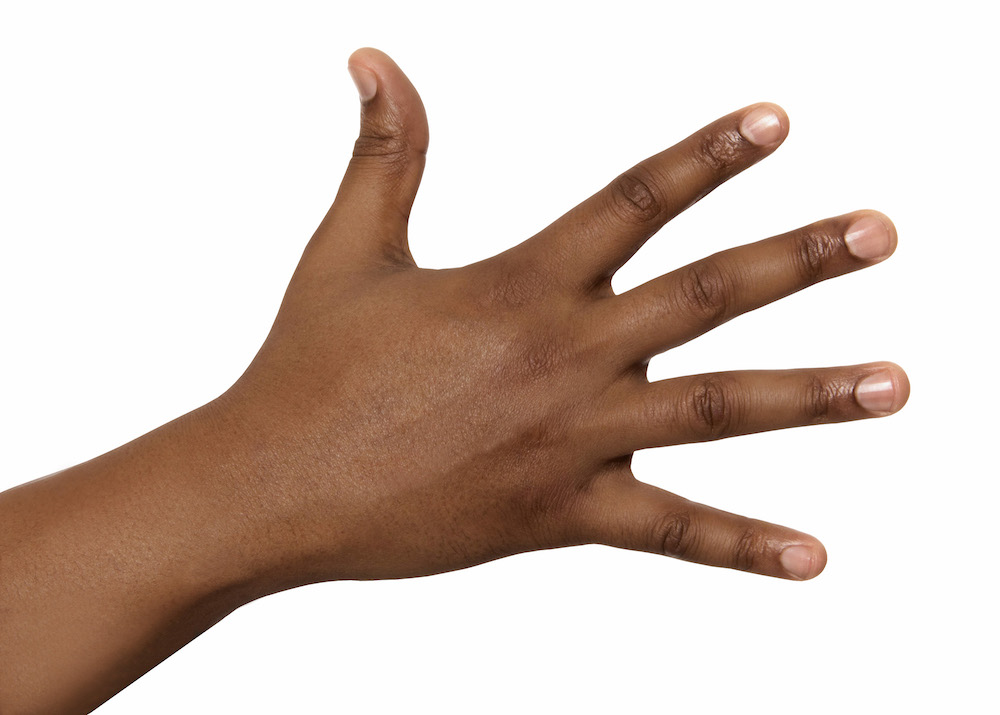
\includegraphics[width=\textwidth,height=\textheight,keepaspectratio]{../inputs/hand_dark.jpg}
  \end{minipage} & 
  \begin{minipage}{.29\textwidth}
    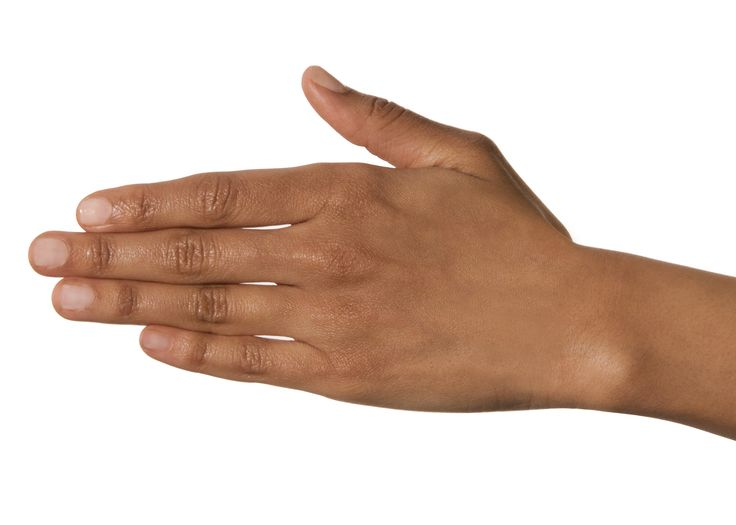
\includegraphics[width=\textwidth,height=\textheight,keepaspectratio]{../inputs/hand_brown.jpg}
  \end{minipage} & 
  \begin{minipage}{.29\textwidth}
    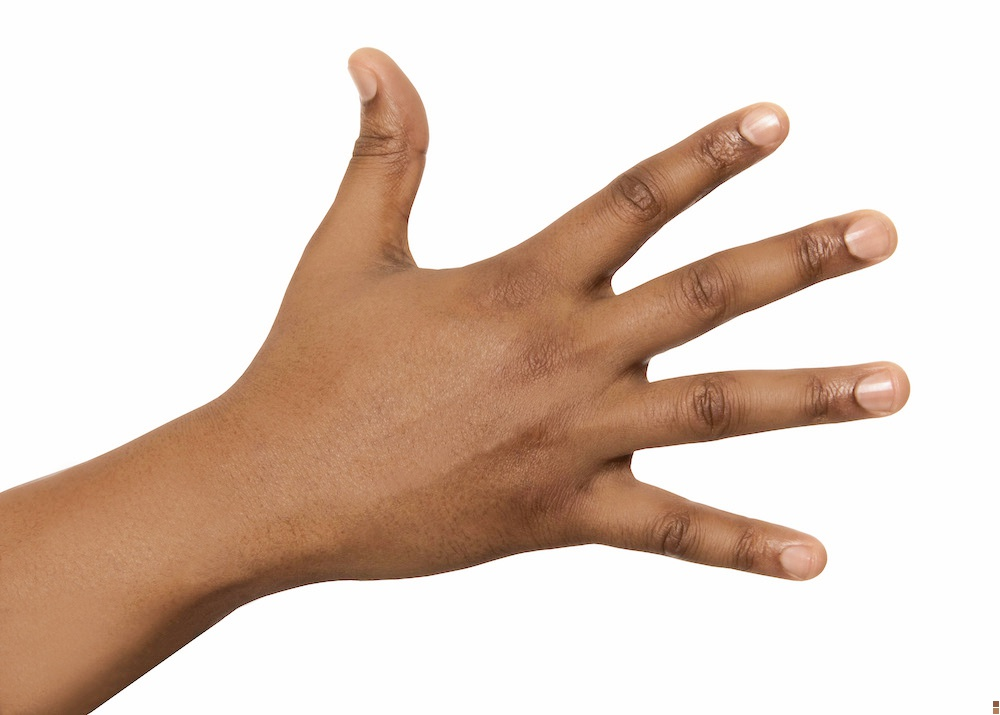
\includegraphics[width=\textwidth,height=\textheight,keepaspectratio]{../rc_test/outputs/20170524_prop_corr_1p1_ave_5/hand_dark_to_hand_brown.jpg}
  \end{minipage} \\
\hline
	  \label{row:PY_NAME_hand_dark_to_hand_light} &
  \begin{minipage}{.29\textwidth}
    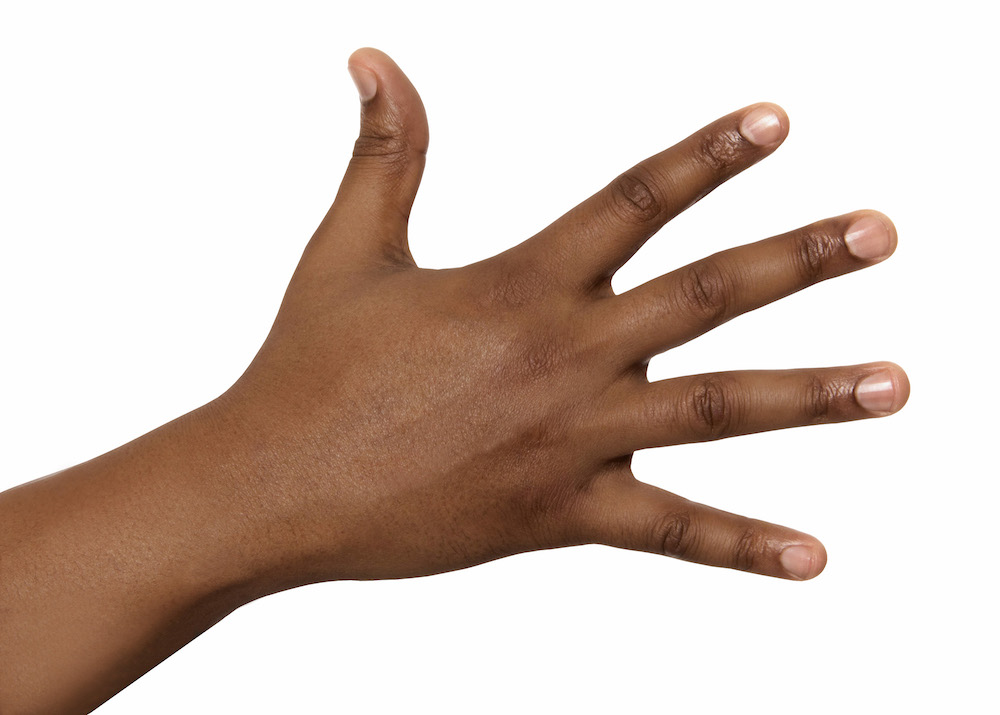
\includegraphics[width=\textwidth,height=\textheight,keepaspectratio]{../inputs/hand_dark.jpg}
  \end{minipage} & 
  \begin{minipage}{.29\textwidth}
    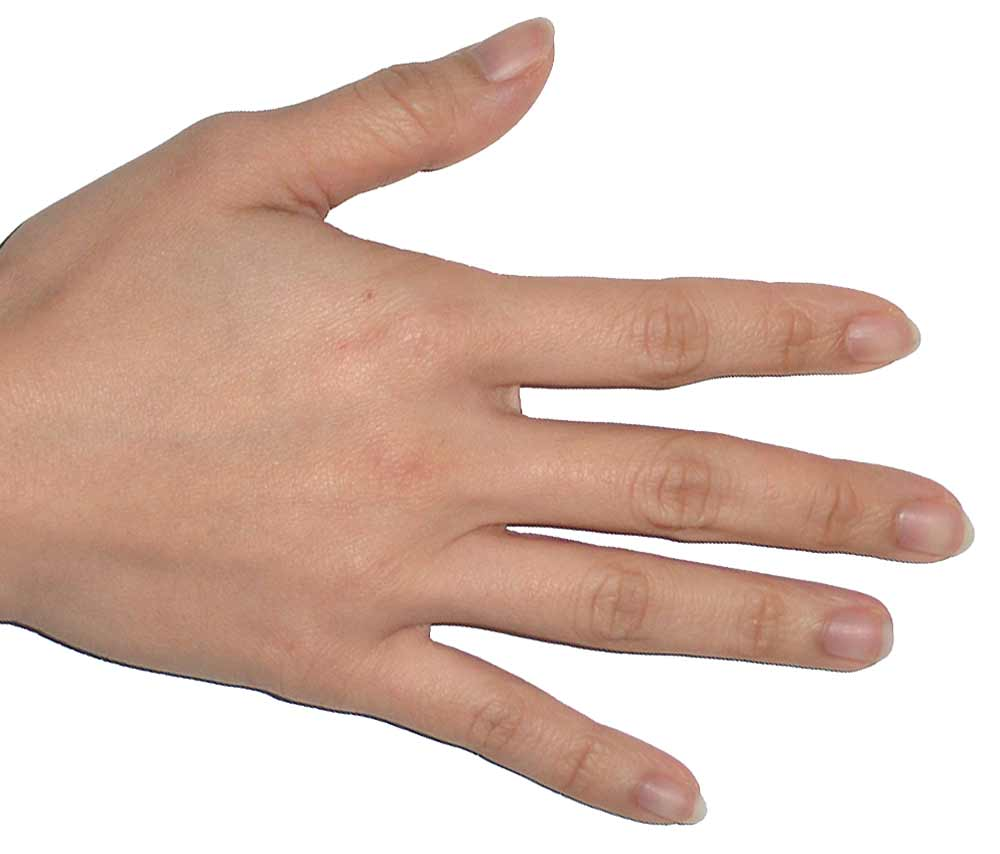
\includegraphics[width=\textwidth,height=\textheight,keepaspectratio]{../inputs/hand_light.jpg}
  \end{minipage} & 
  \begin{minipage}{.29\textwidth}
    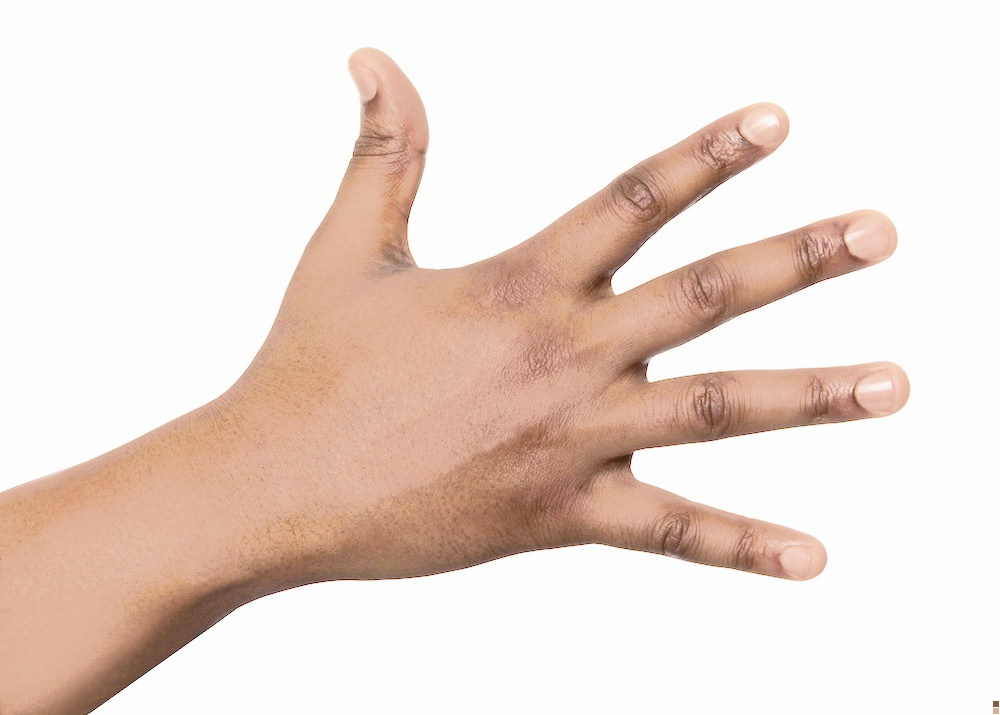
\includegraphics[width=\textwidth,height=\textheight,keepaspectratio]{../rc_test/outputs/20170524_prop_corr_1p1_ave_5/hand_dark_to_hand_light.jpg}
  \end{minipage} \\
\hline
	  \label{row:PY_NAME_hand_dark_to_hand_pale} &
  \begin{minipage}{.29\textwidth}
    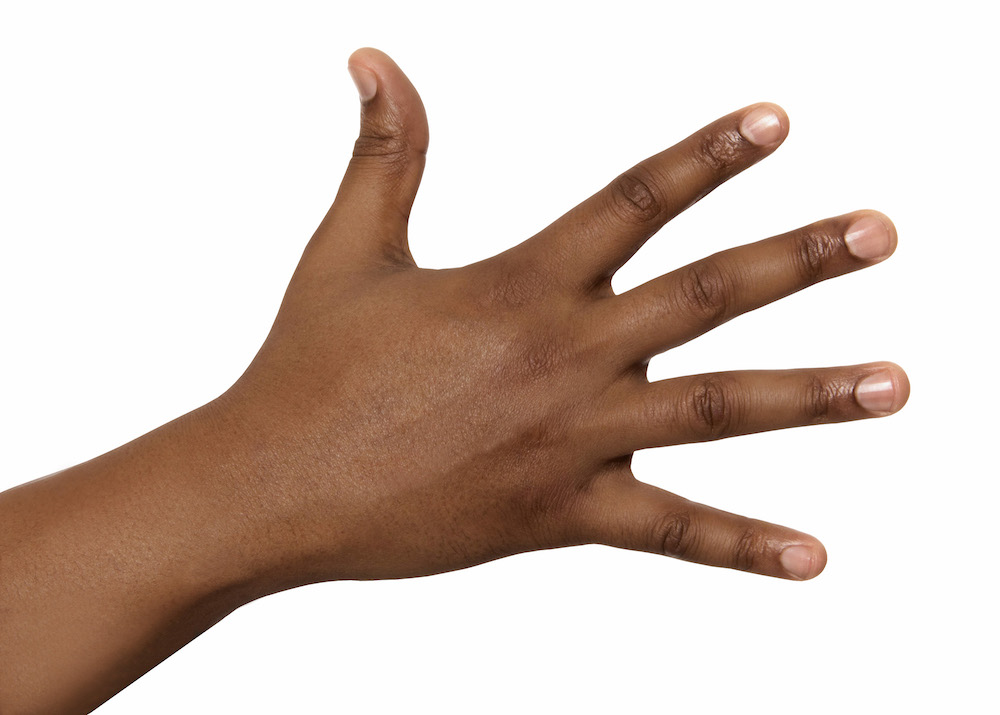
\includegraphics[width=\textwidth,height=\textheight,keepaspectratio]{../inputs/hand_dark.jpg}
  \end{minipage} & 
  \begin{minipage}{.29\textwidth}
    \includegraphics[width=\textwidth,height=\textheight,keepaspectratio]{../inputs/hand_pale.jpg}
  \end{minipage} & 
  \begin{minipage}{.29\textwidth}
    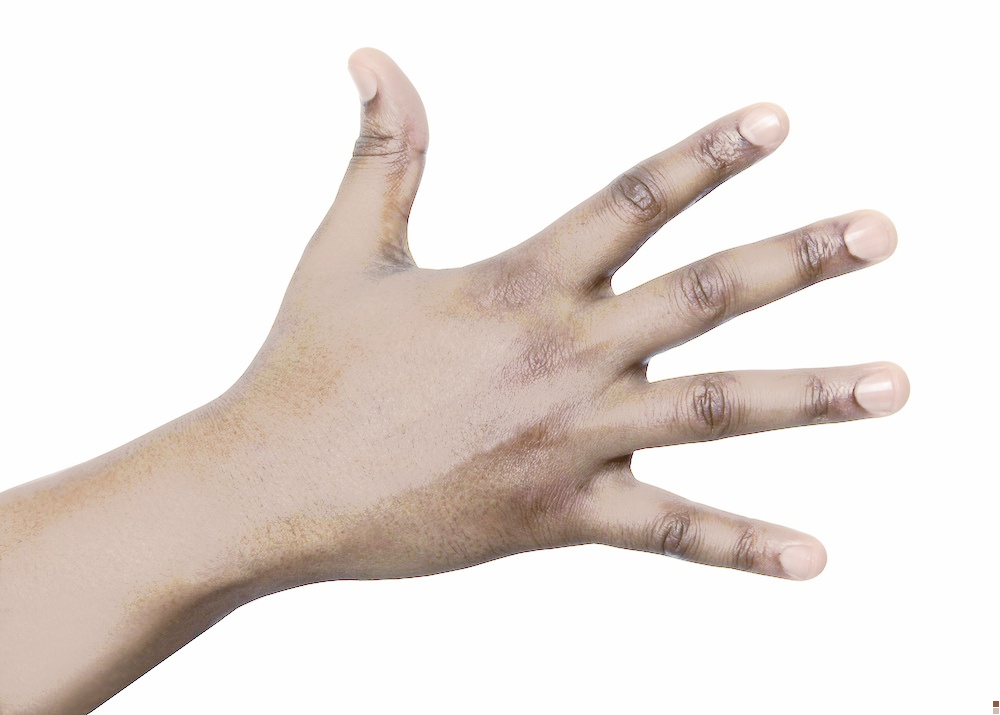
\includegraphics[width=\textwidth,height=\textheight,keepaspectratio]{../rc_test/outputs/20170524_prop_corr_1p1_ave_5/hand_dark_to_hand_pale.jpg}
  \end{minipage} \\
\hline
	  \label{row:PY_NAME_hand_brown_to_hand_dark} &
  \begin{minipage}{.29\textwidth}
    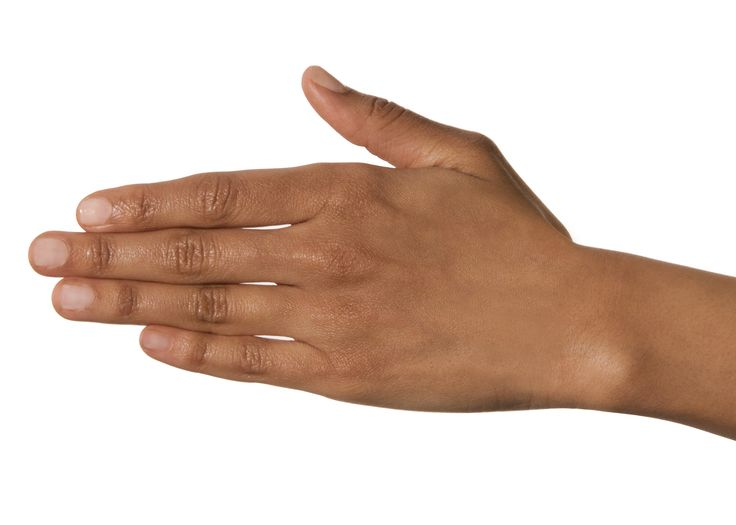
\includegraphics[width=\textwidth,height=\textheight,keepaspectratio]{../inputs/hand_brown.jpg}
  \end{minipage} & 
  \begin{minipage}{.29\textwidth}
    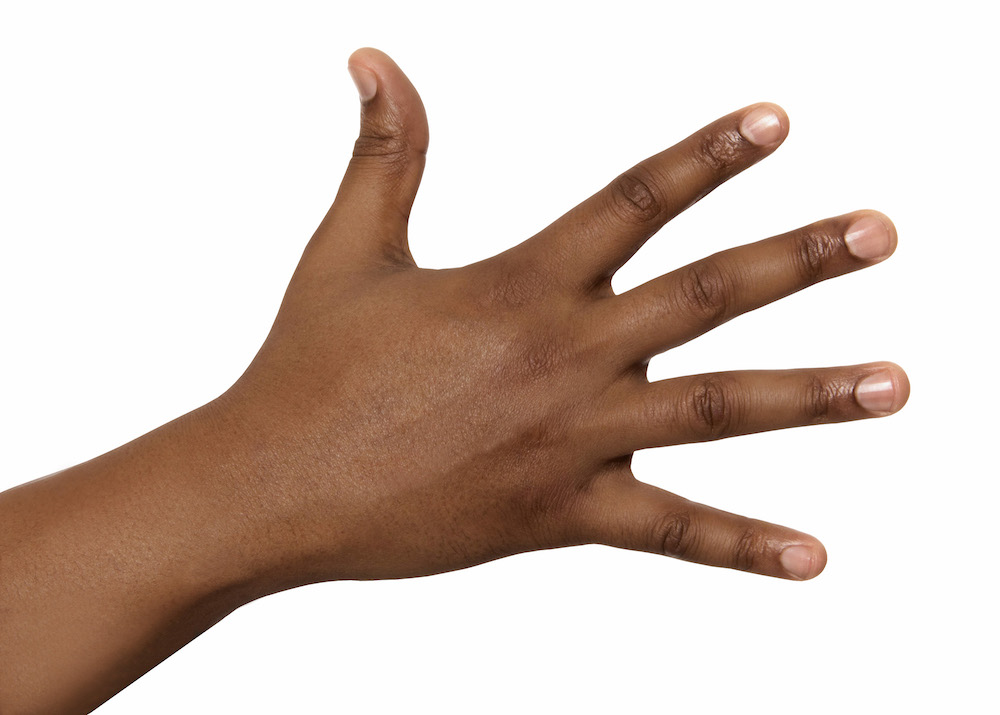
\includegraphics[width=\textwidth,height=\textheight,keepaspectratio]{../inputs/hand_dark.jpg}
  \end{minipage} & 
  \begin{minipage}{.29\textwidth}
    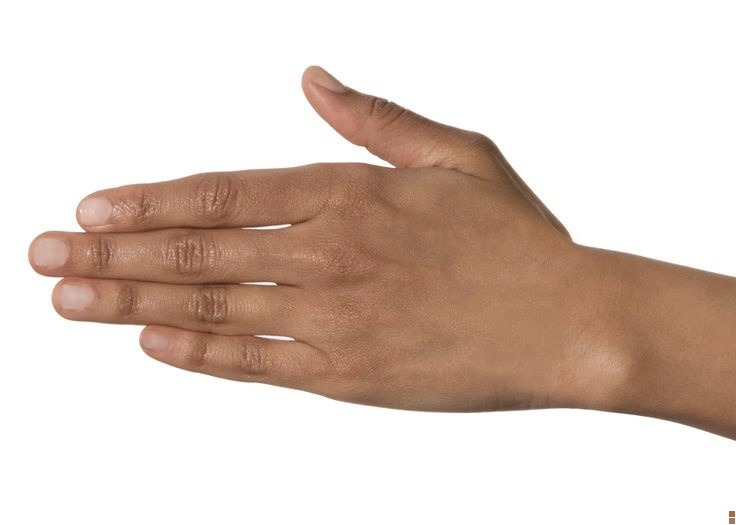
\includegraphics[width=\textwidth,height=\textheight,keepaspectratio]{../rc_test/outputs/20170524_prop_corr_1p1_ave_10/hand_brown_to_hand_dark.jpg}
  \end{minipage} \\
\hline
	  \label{row:PY_NAME_hand_brown_to_hand_light} &
  \begin{minipage}{.29\textwidth}
    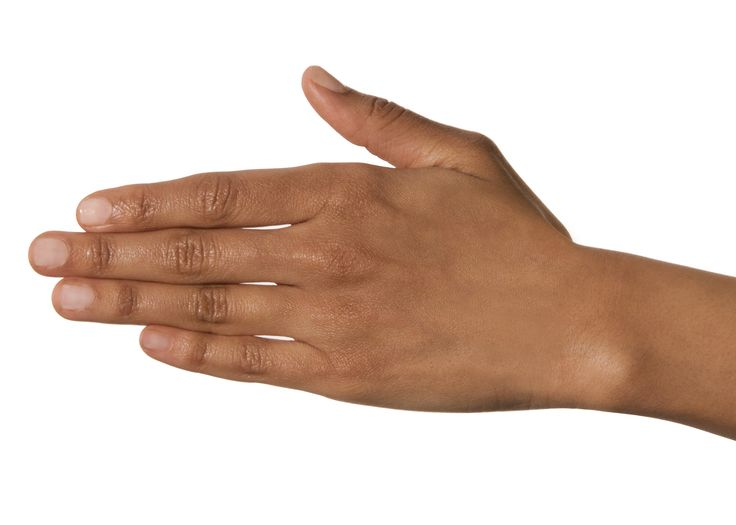
\includegraphics[width=\textwidth,height=\textheight,keepaspectratio]{../inputs/hand_brown.jpg}
  \end{minipage} & 
  \begin{minipage}{.29\textwidth}
    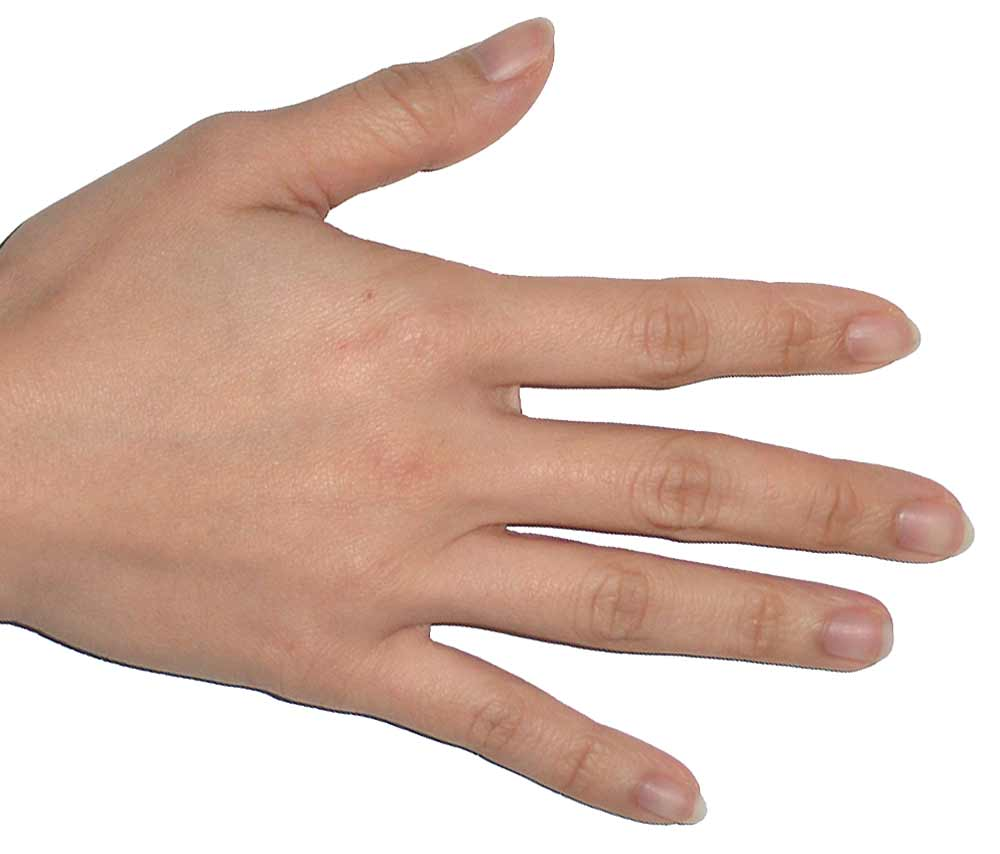
\includegraphics[width=\textwidth,height=\textheight,keepaspectratio]{../inputs/hand_light.jpg}
  \end{minipage} & 
  \begin{minipage}{.29\textwidth}
    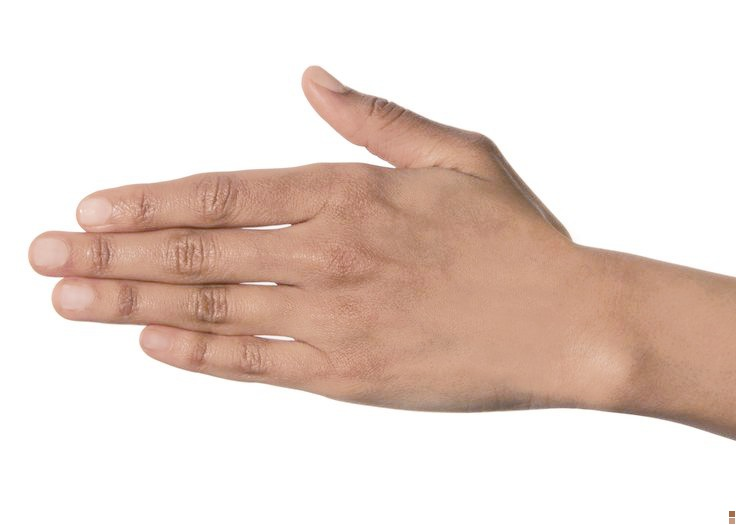
\includegraphics[width=\textwidth,height=\textheight,keepaspectratio]{../rc_test/outputs/20170524_prop_corr_1p1_ave_100/hand_brown_to_hand_light.jpg}
  \end{minipage} \\
\hline
	  \ref{row:PY_NAME_hand_brown_to_hand_pale} &
  \begin{minipage}{.29\textwidth}
    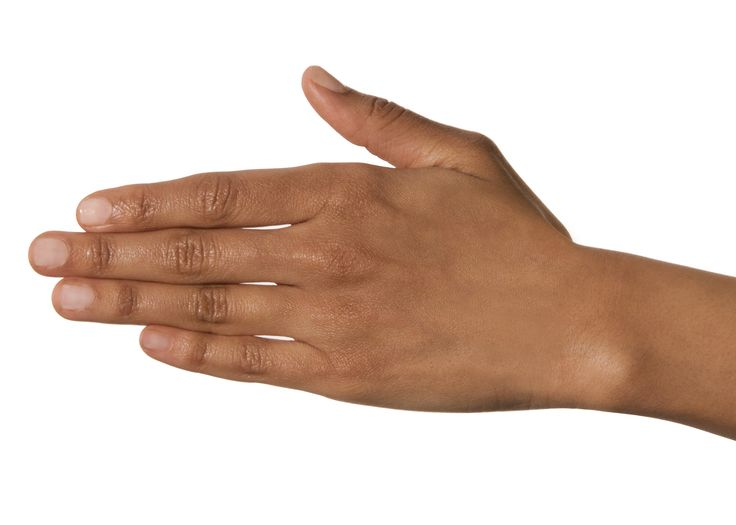
\includegraphics[width=\textwidth,height=\textheight,keepaspectratio]{../inputs/hand_brown.jpg}
  \end{minipage} & 
  \begin{minipage}{.29\textwidth}
    \includegraphics[width=\textwidth,height=\textheight,keepaspectratio]{../inputs/hand_pale.jpg}
  \end{minipage} & 
  \begin{minipage}{.29\textwidth}
    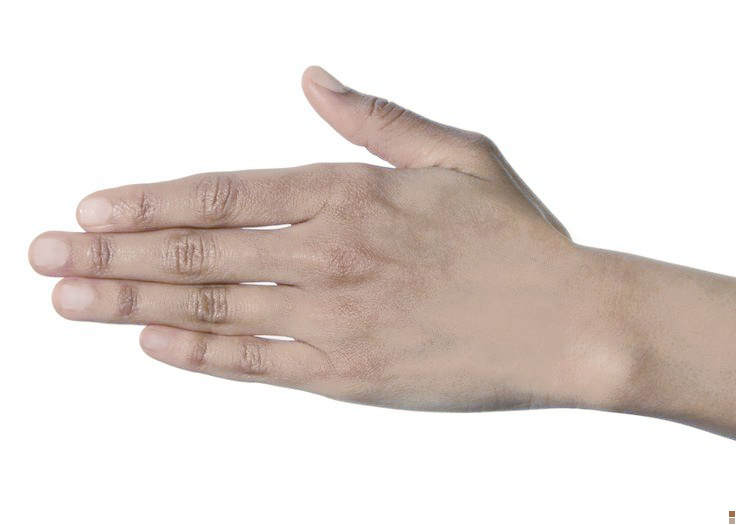
\includegraphics[width=\textwidth,height=\textheight,keepaspectratio]{../rc_test/outputs/20170524_prop_corr_1p1_ave_25/hand_brown_to_hand_pale.jpg}
  \end{minipage} \\
\hline
	  \label{row:PY_NAME_hand_light_to_hand_dark} &
  \begin{minipage}{.29\textwidth}
    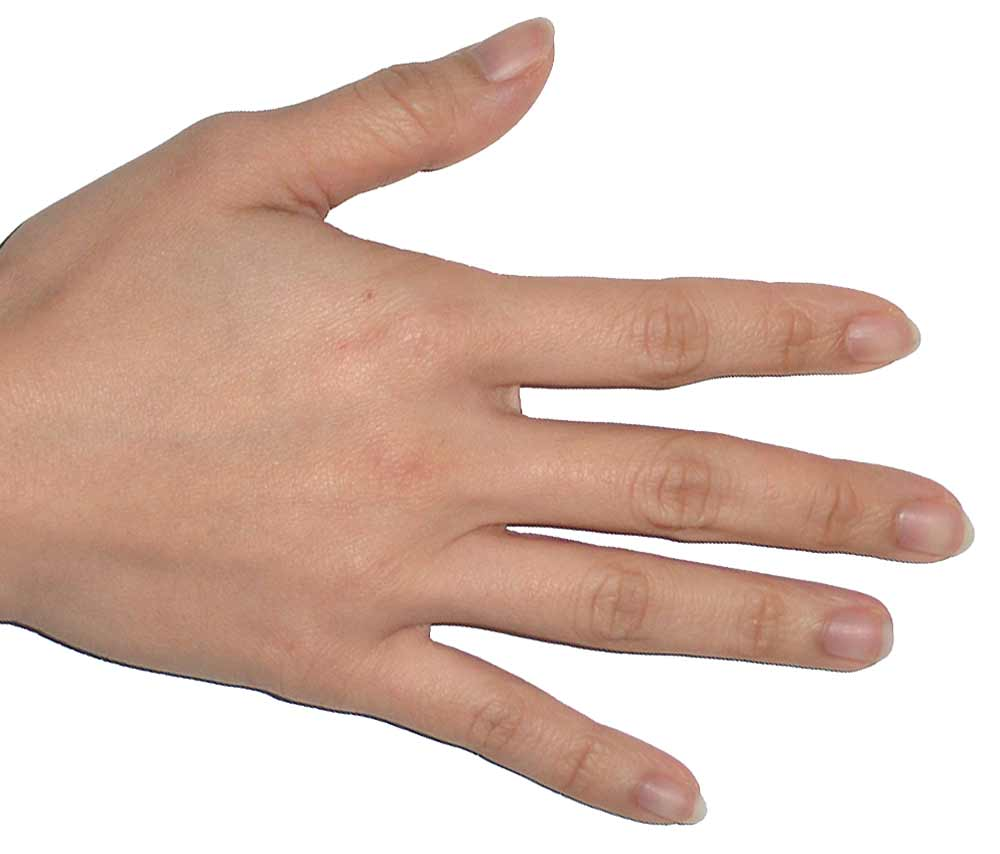
\includegraphics[width=\textwidth,height=\textheight,keepaspectratio]{../inputs/hand_light.jpg}
  \end{minipage} & 
  \begin{minipage}{.29\textwidth}
    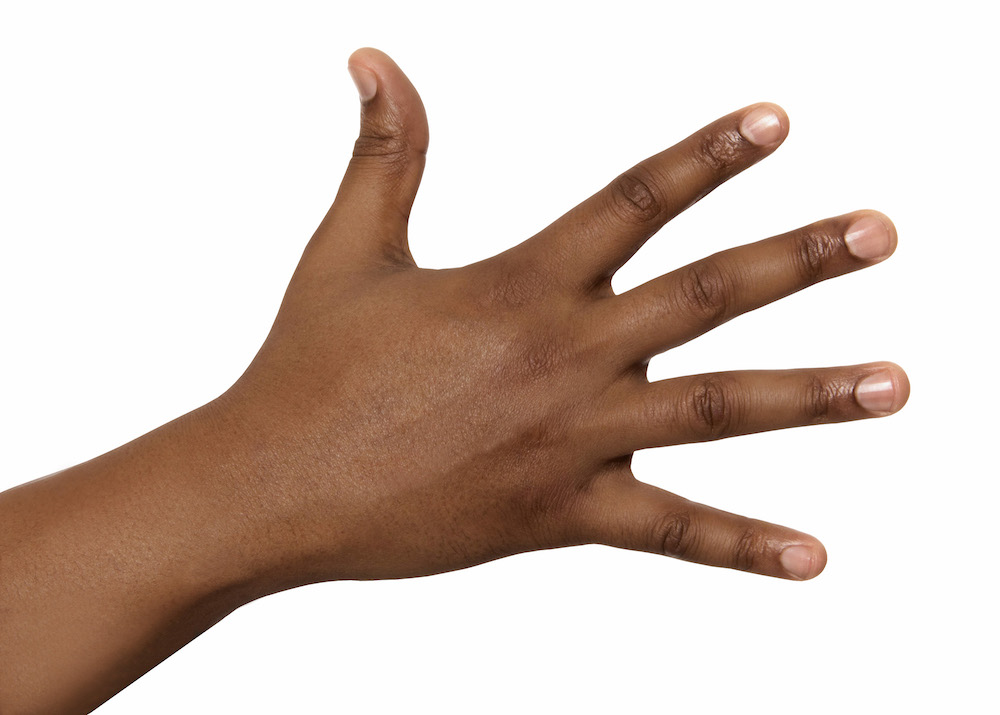
\includegraphics[width=\textwidth,height=\textheight,keepaspectratio]{../inputs/hand_dark.jpg}
  \end{minipage} & 
  \begin{minipage}{.29\textwidth}
    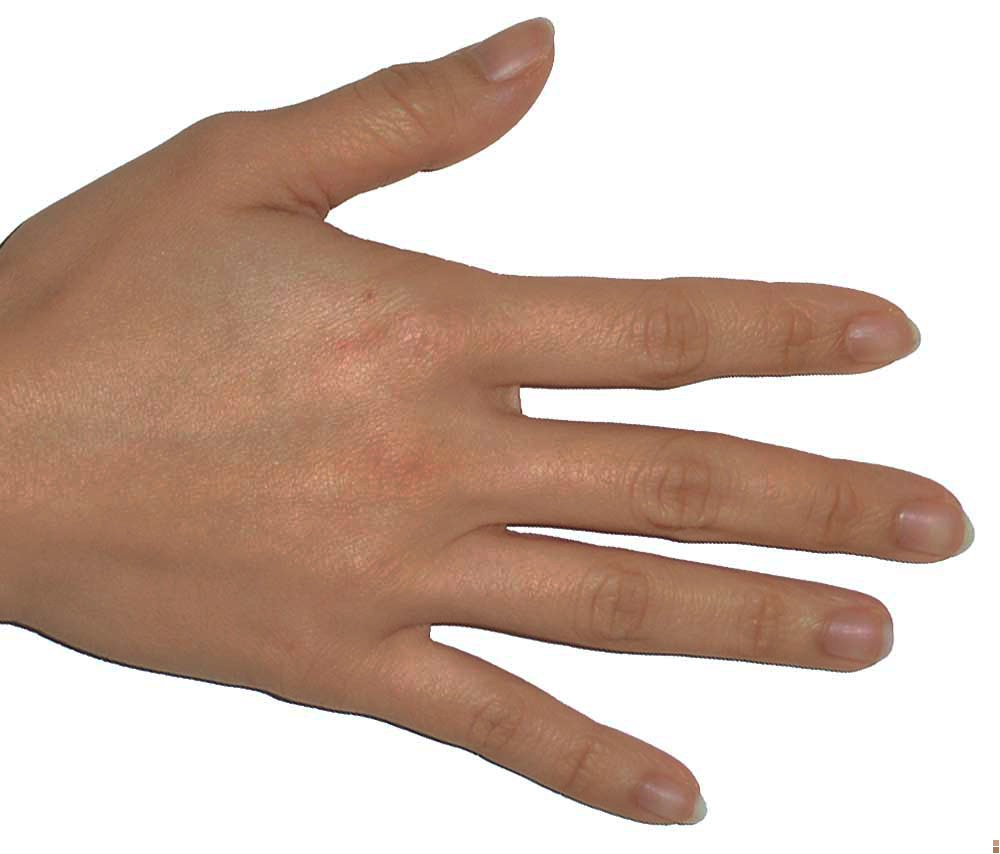
\includegraphics[width=\textwidth,height=\textheight,keepaspectratio]{../rc_test/outputs/20170524_prop_corr_1p1_ave_5/hand_light_to_hand_dark.jpg}
  \end{minipage} \\
\hline
	  \label{row:PY_NAME_hand_light_to_hand_brown} &
  \begin{minipage}{.29\textwidth}
    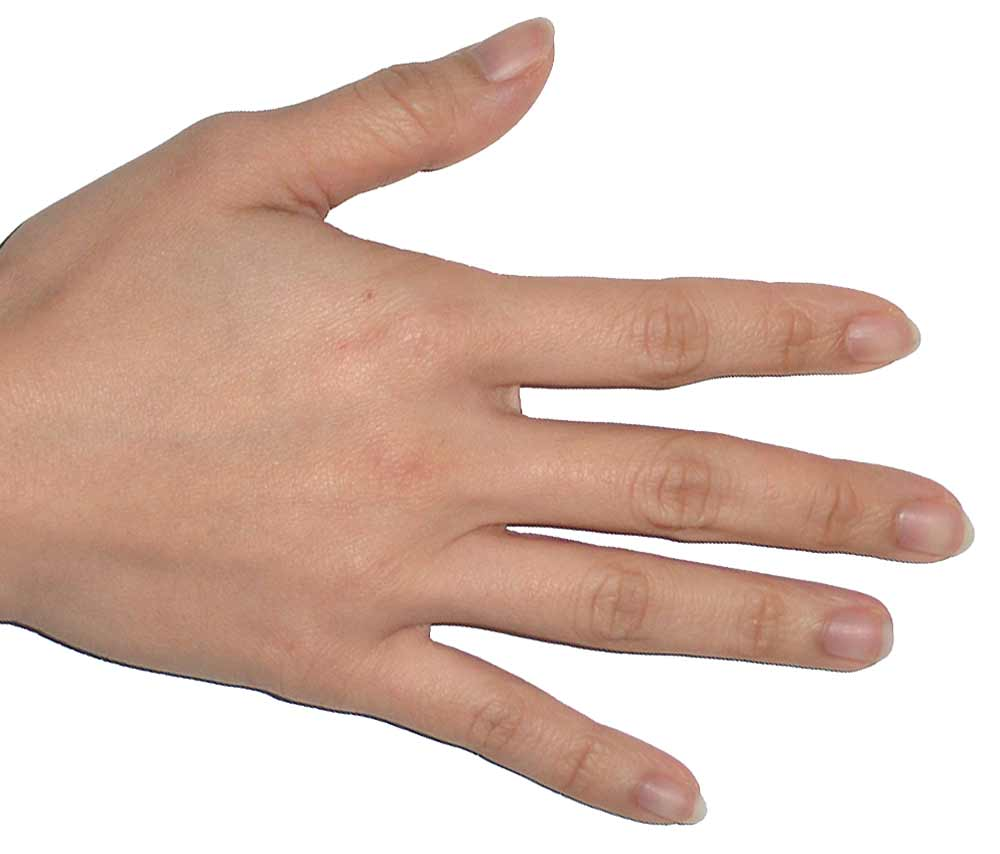
\includegraphics[width=\textwidth,height=\textheight,keepaspectratio]{../inputs/hand_light.jpg}
  \end{minipage} & 
  \begin{minipage}{.29\textwidth}
    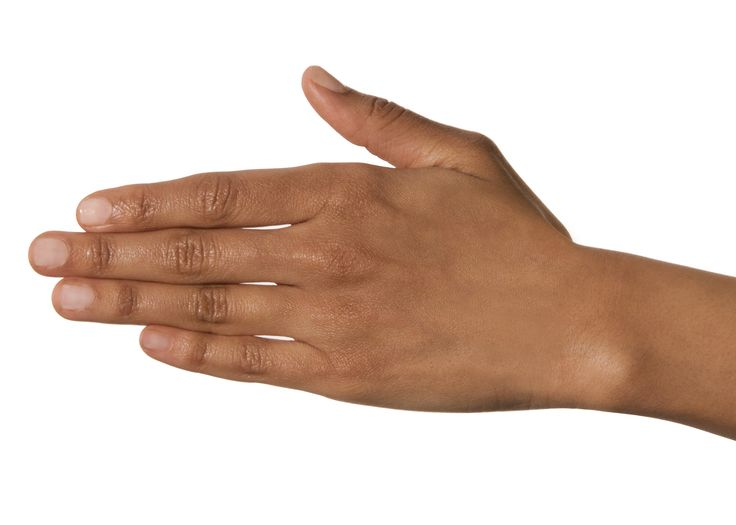
\includegraphics[width=\textwidth,height=\textheight,keepaspectratio]{../inputs/hand_brown.jpg}
  \end{minipage} & 
  \begin{minipage}{.29\textwidth}
    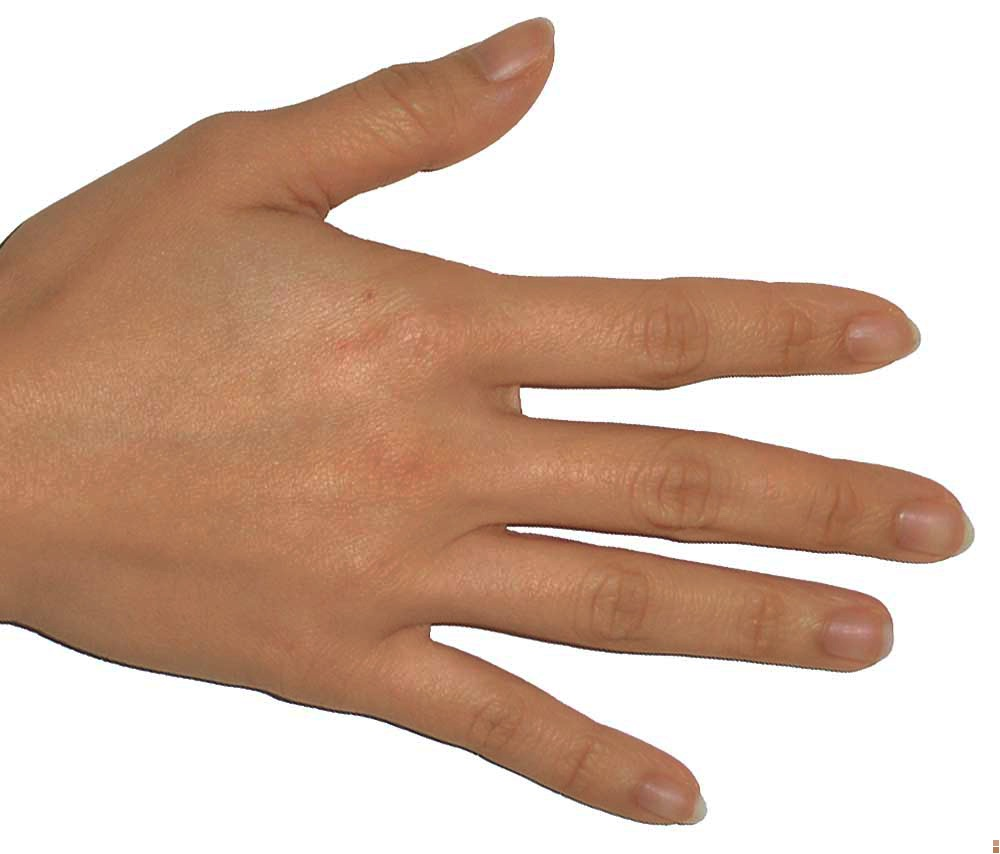
\includegraphics[width=\textwidth,height=\textheight,keepaspectratio]{../rc_test/outputs/20170524_prop_corr_1p1_ave_5/hand_light_to_hand_brown.jpg}
  \end{minipage} \\
\hline
	  \label{row:PY_NAME_hand_light_to_hand_pale} &
  \begin{minipage}{.29\textwidth}
    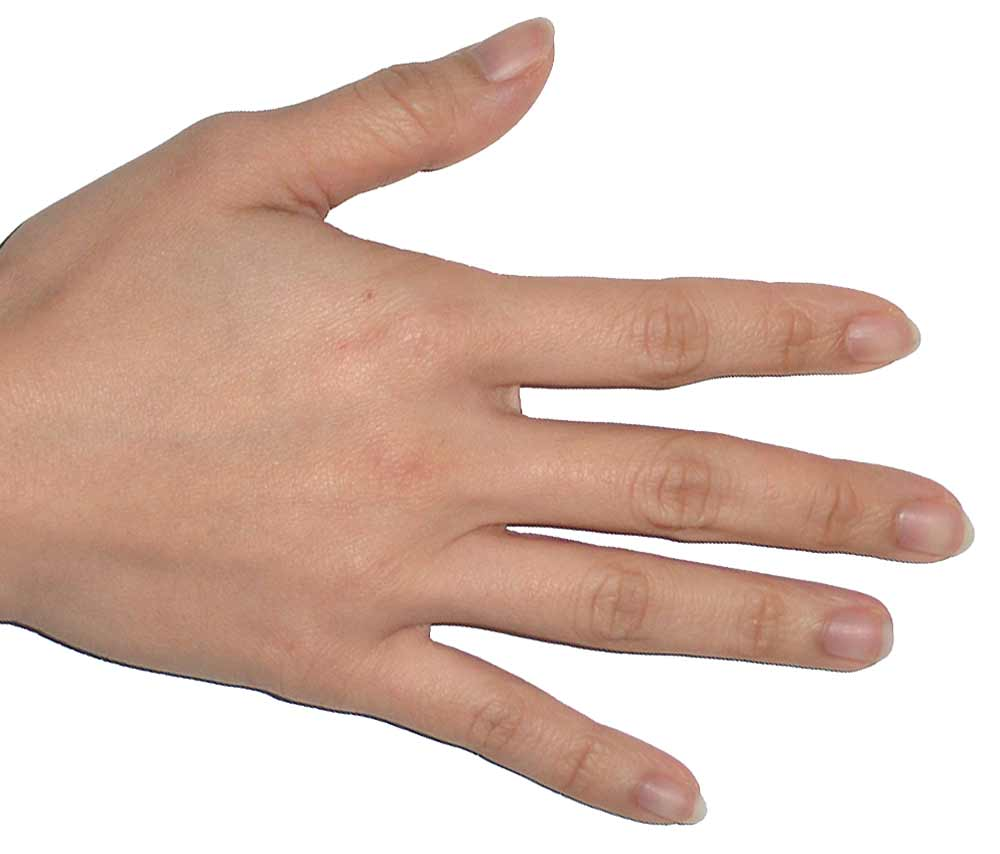
\includegraphics[width=\textwidth,height=\textheight,keepaspectratio]{../inputs/hand_light.jpg}
  \end{minipage} & 
  \begin{minipage}{.29\textwidth}
    \includegraphics[width=\textwidth,height=\textheight,keepaspectratio]{../inputs/hand_pale.jpg}
  \end{minipage} & 
  \begin{minipage}{.29\textwidth}
    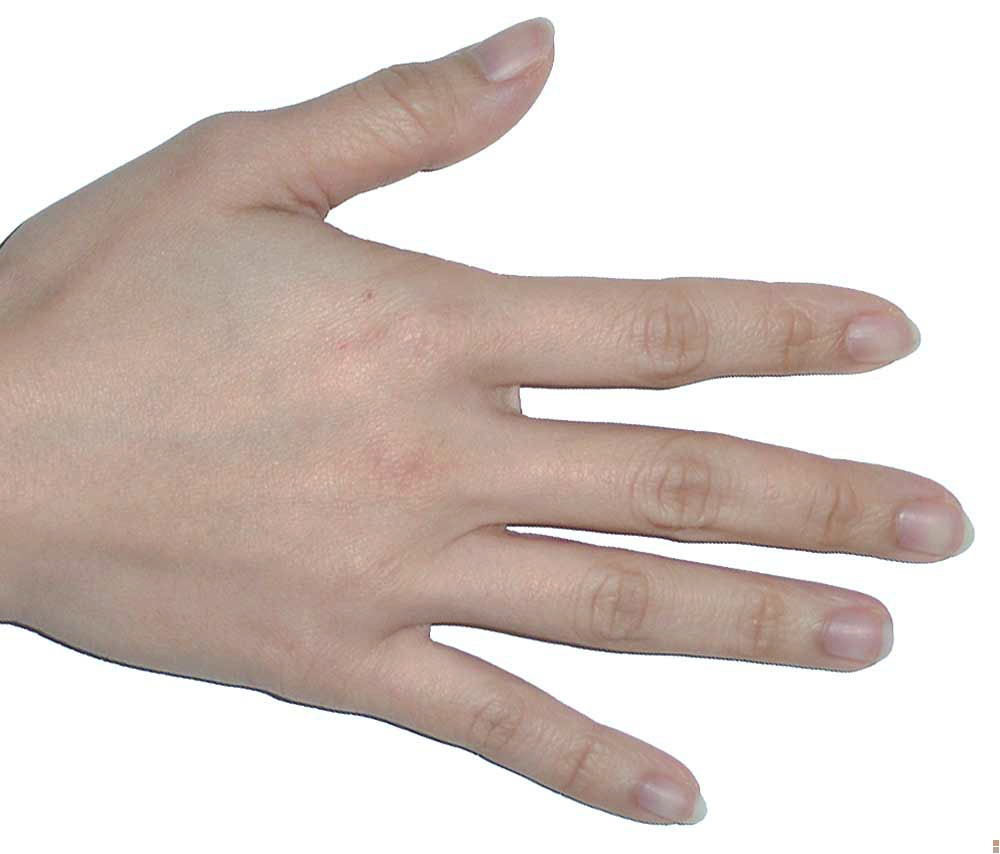
\includegraphics[width=\textwidth,height=\textheight,keepaspectratio]{../rc_test/outputs/20170524_prop_corr_1p1_ave_25/hand_light_to_hand_pale.jpg}
  \end{minipage} \\
\hline
	  \ref{row:PY_NAME_hand_pale_to_hand_dark} &
  \begin{minipage}{.29\textwidth}
    \includegraphics[width=\textwidth,height=\textheight,keepaspectratio]{../inputs/hand_pale.jpg}
  \end{minipage} & 
  \begin{minipage}{.29\textwidth}
    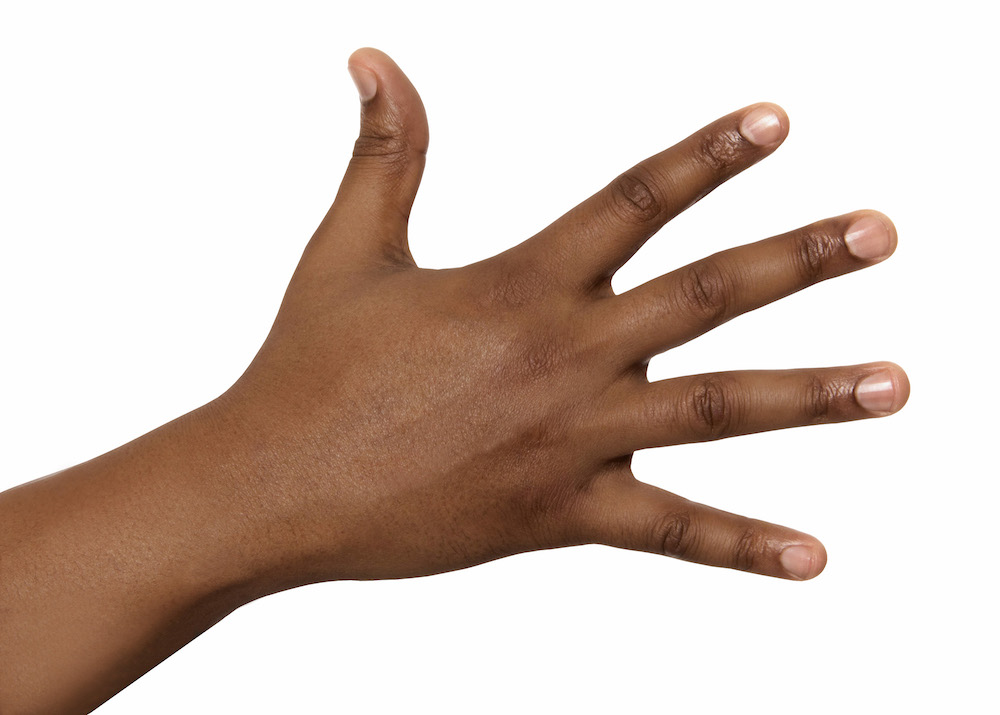
\includegraphics[width=\textwidth,height=\textheight,keepaspectratio]{../inputs/hand_dark.jpg}
  \end{minipage} & 
  \begin{minipage}{.29\textwidth}
    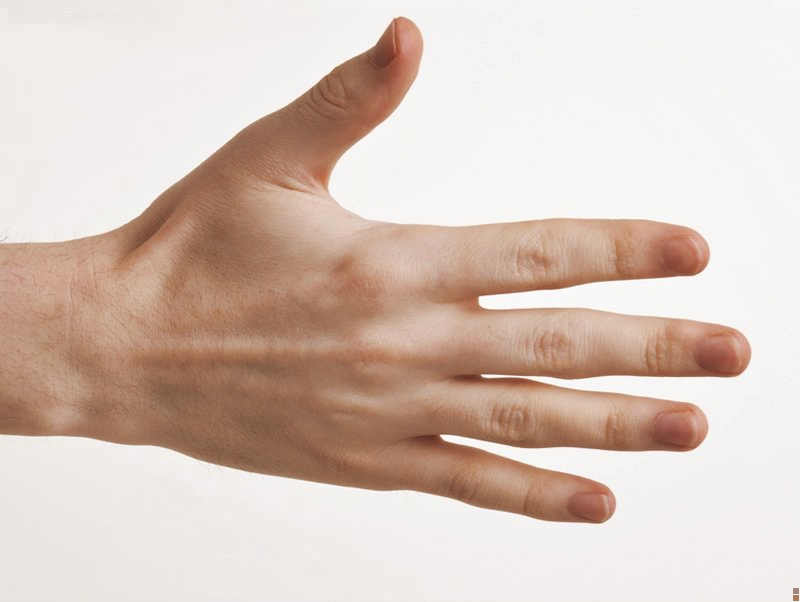
\includegraphics[width=\textwidth,height=\textheight,keepaspectratio]{../rc_test/outputs/20170524_prop_corr_1p1_ave_5/hand_pale_to_hand_dark.jpg}
  \end{minipage} \\
\hline
	  \ref{row:PY_NAME_hand_pale_to_hand_brown} &
  \begin{minipage}{.29\textwidth}
    \includegraphics[width=\textwidth,height=\textheight,keepaspectratio]{../inputs/hand_pale.jpg}
  \end{minipage} & 
  \begin{minipage}{.29\textwidth}
    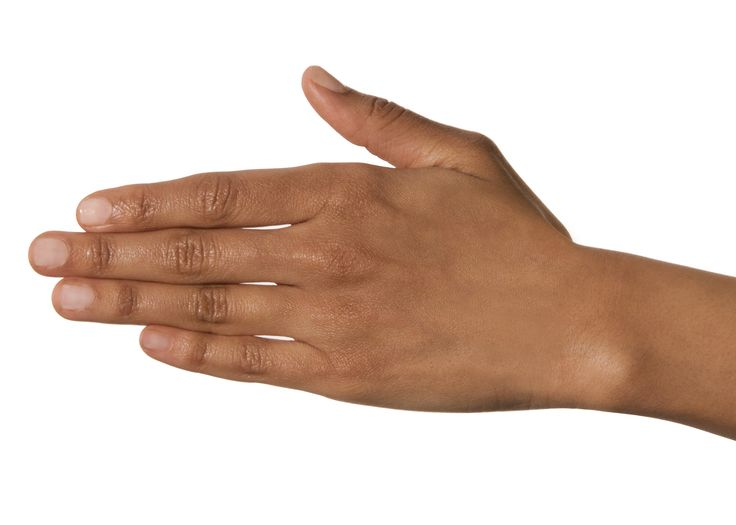
\includegraphics[width=\textwidth,height=\textheight,keepaspectratio]{../inputs/hand_brown.jpg}
  \end{minipage} & 
  \begin{minipage}{.29\textwidth}
    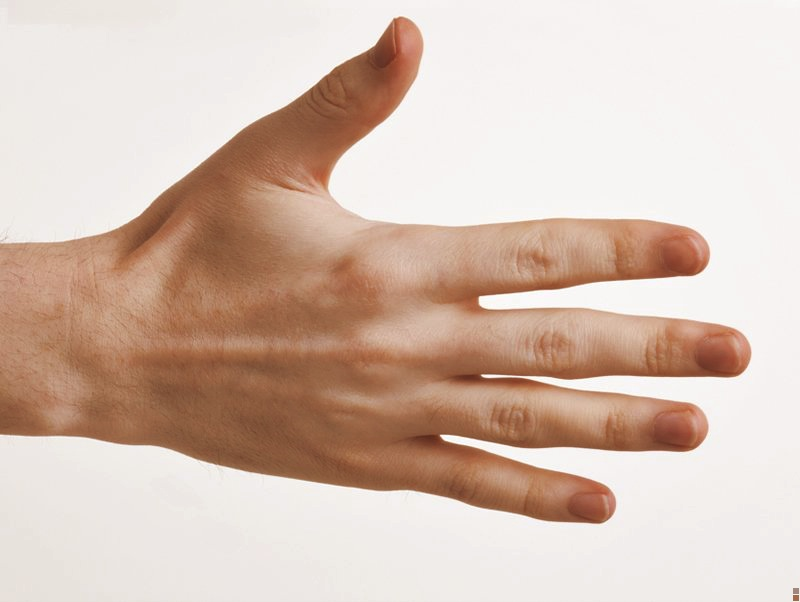
\includegraphics[width=\textwidth,height=\textheight,keepaspectratio]{../rc_test/outputs/20170524_prop_corr_1p1_ave_100/hand_pale_to_hand_brown.jpg}
  \end{minipage} \\
\hline
	  \ref{row:PY_NAME_hand_pale_to_hand_light} &
  \begin{minipage}{.29\textwidth}
    \includegraphics[width=\textwidth,height=\textheight,keepaspectratio]{../inputs/hand_pale.jpg}
  \end{minipage} & 
  \begin{minipage}{.29\textwidth}
    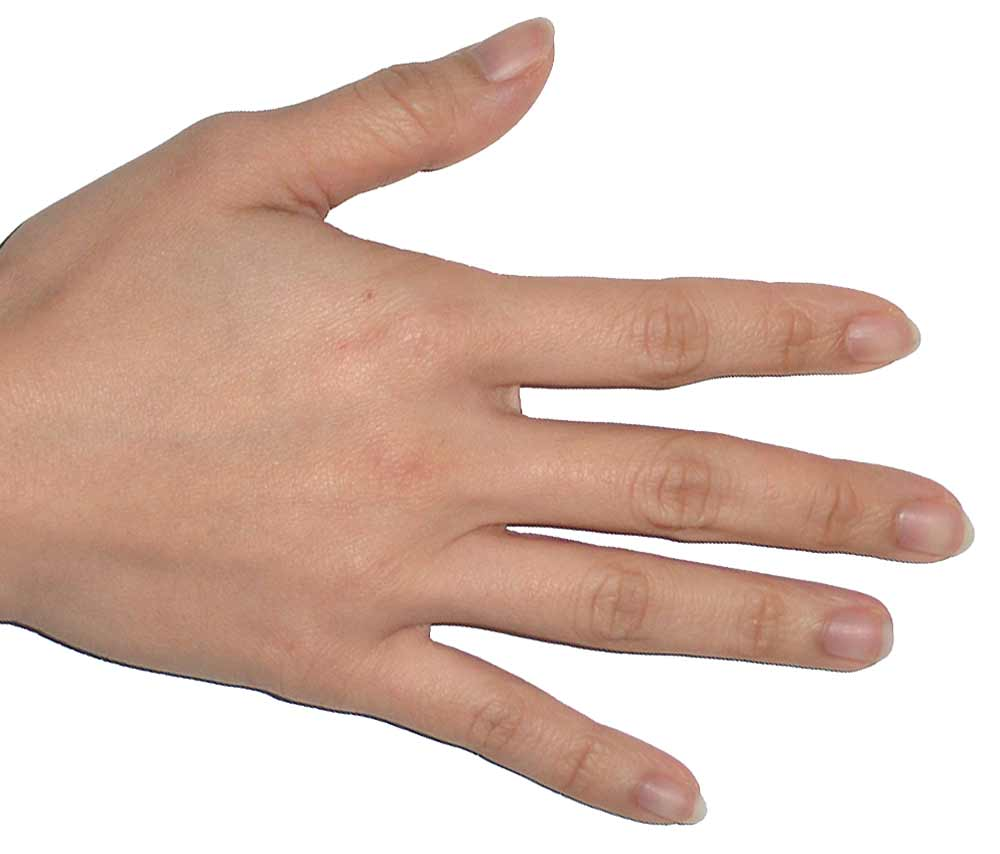
\includegraphics[width=\textwidth,height=\textheight,keepaspectratio]{../inputs/hand_light.jpg}
  \end{minipage} & 
  \begin{minipage}{.29\textwidth}
    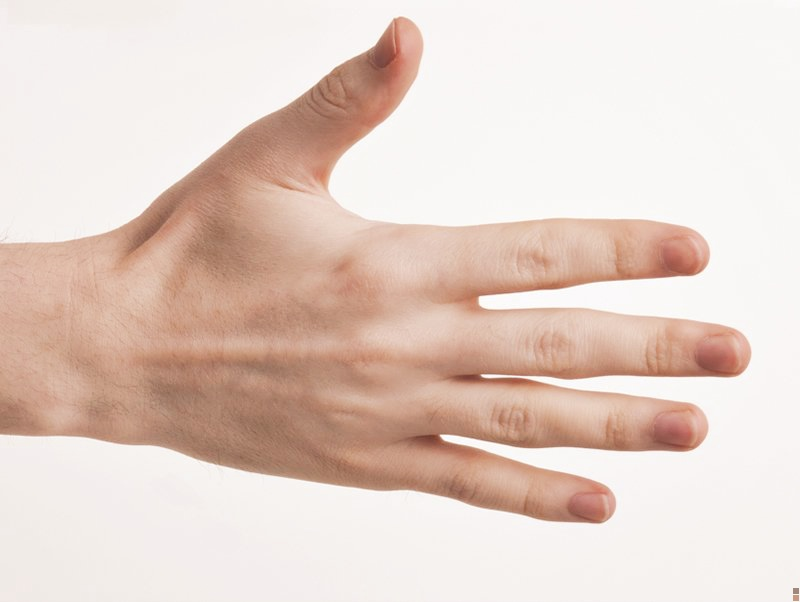
\includegraphics[width=\textwidth,height=\textheight,keepaspectratio]{../rc_test/outputs/20170524_prop_corr_1p1_ave_100/hand_pale_to_hand_light.jpg}
  \end{minipage} \\
\hline

 \end{longtable}

\subsubsection*{Evaluation}
Figure \ref{img:10_perc_mask} demonstrates the new regions used to calculate the average skin colour. We can see that the areas with shadows are effectively discarded, and the average colour calculated is significantly lighter and visually closer to the skin colour of the target hand. 

\begin{figure}[H]
\centering
\begin{tabular}{ccc}
    \multirow{2}{*}[5em]{\begin{subfigure}[b]{0.30\textwidth}
        \includegraphics[width=\textwidth]{images/hand_pale}
        \caption{Input hand image with significant shadows}\label{img:alg_3_eval_hand_pale}
    \end{subfigure}}&
    \begin{subfigure}[b]{0.30\textwidth}
        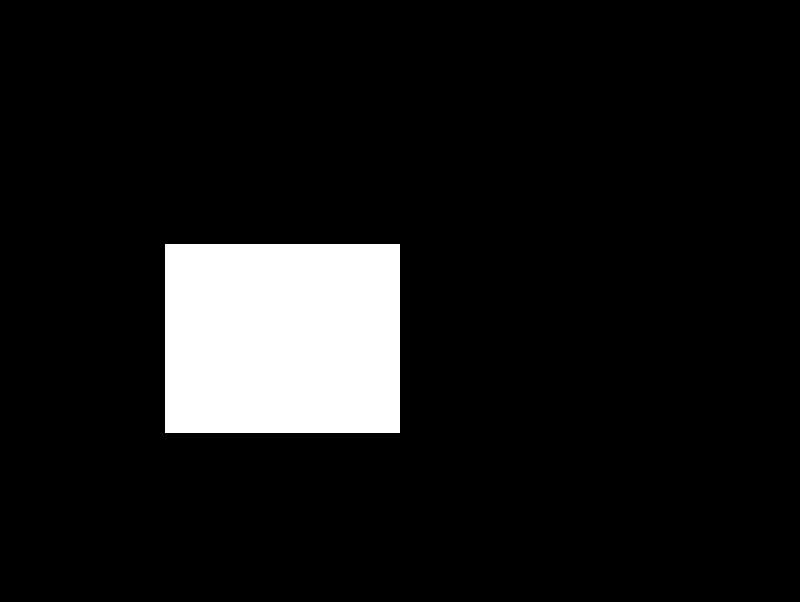
\includegraphics[width=\textwidth]{images/pale_ave_10_original_mask}
        \caption{Mask used to calculate color in Algorithm \ref{eq:prop_corr_algo}}\label{img:original_mask}
    \end{subfigure} &
    \begin{subfigure}[b]{0.30\textwidth}
        
\includegraphics[width=\textwidth]{images/ave_col_100}
        \caption{Average color calculated with Algorithm \ref{eq:prop_corr_algo}}\label{img:ave_col_100}
    \end{subfigure}\\
    &
    \begin{subfigure}[b]{0.30\textwidth}
        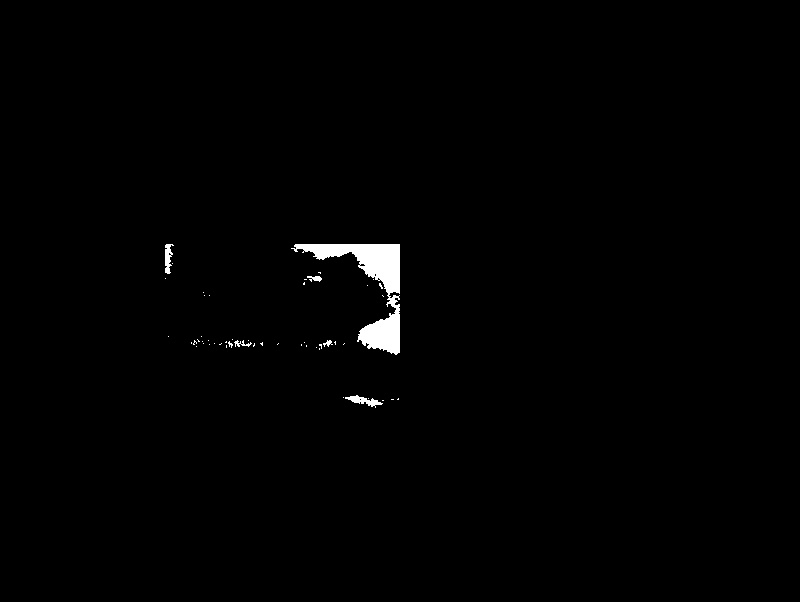
\includegraphics[width=\textwidth]{images/pale_ave_10_adjusted_mask}
        \caption{Mask used to calculate color in Algorithm \ref{eq:prop_corr_ave_algo}}\label{img:adjusted_mask}
    \end{subfigure} &
    \begin{subfigure}[b]{0.30\textwidth}
        
\includegraphics[width=\textwidth]{images/ave_col_10}
        \caption{Average color calculated with Algorithm \ref{eq:prop_corr_ave_algo}}\label{img:ave_col_10}
    \end{subfigure}
\end{tabular}
\caption{The average color calculation process in Algorithm \ref{eq:prop_corr_ave_algo} compared the previous version, Algorithm \ref{eq:prop_corr_algo}}\label{img:10_perc_mask}
\end{figure}